\appendix
\chapter{}
\addcontentsline{toc}{chapter}{Anhang A}
\section{Ergebnisse aus dem Landscape Datensatz}
\begin{figure}[H]
  \centering
  \vspace{1cm}
  \begin{subfigure}
    \centering
    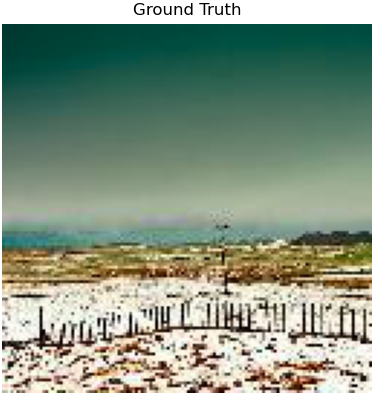
\includegraphics[width=.235\textwidth]{resources/experiments/landscape/324_bins/273/273_original.png}
  \end{subfigure}
  \begin{subfigure}
    \centering
    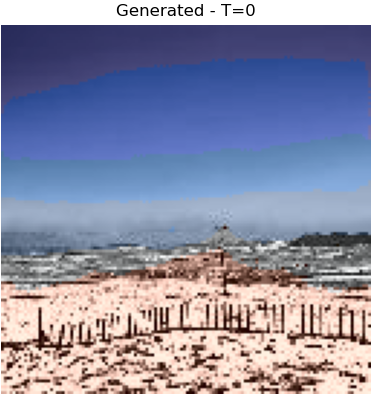
\includegraphics[width=.235\textwidth]{resources/experiments/landscape/324_bins/273/273_t0.png}
  \end{subfigure}
  \begin{subfigure}
    \centering
    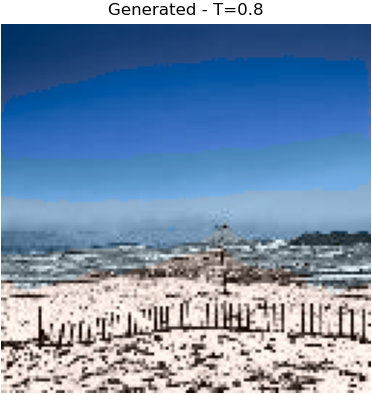
\includegraphics[width=.235\textwidth]{resources/experiments/landscape/324_bins/273/273_t08.png}
  \end{subfigure}
  \begin{subfigure}
    \centering
    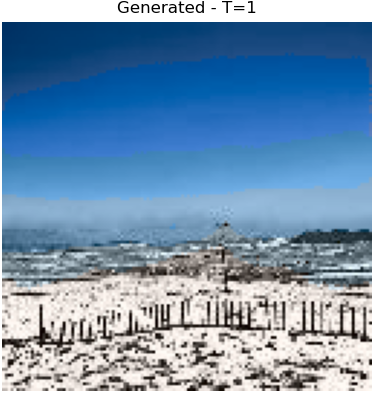
\includegraphics[width=.235\textwidth]{resources/experiments/landscape/324_bins/273/273_t1.png}
  \end{subfigure}

  \begin{subfigure}
    \centering
    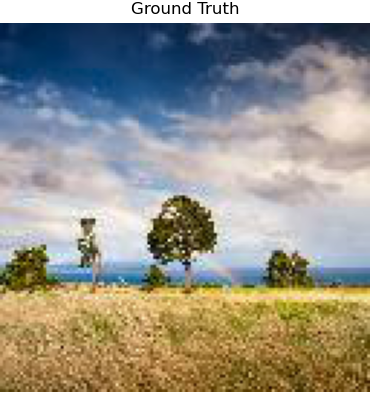
\includegraphics[width=.235\textwidth]{resources/experiments/landscape/324_bins/280/280_original.png}
  \end{subfigure}
  \begin{subfigure}
    \centering
    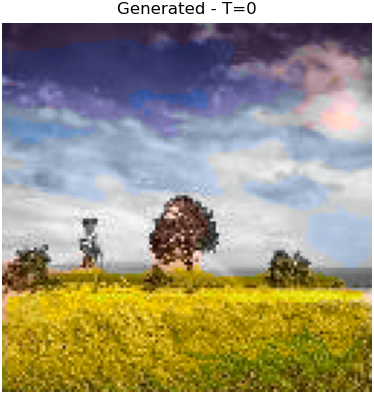
\includegraphics[width=.235\textwidth]{resources/experiments/landscape/324_bins/280/280_t0.png}
  \end{subfigure}
  \begin{subfigure}
    \centering
    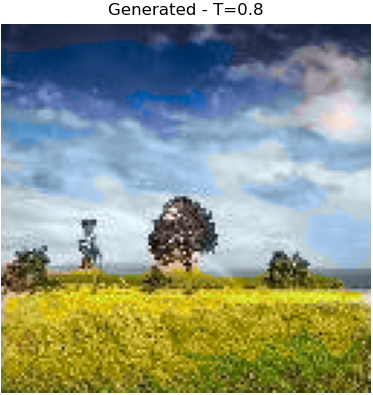
\includegraphics[width=.235\textwidth]{resources/experiments/landscape/324_bins/280/280_t08.png}
  \end{subfigure}
  \begin{subfigure}
    \centering
    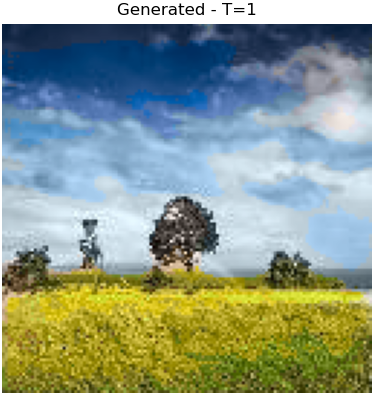
\includegraphics[width=.235\textwidth]{resources/experiments/landscape/324_bins/280/280_t1.png}
  \end{subfigure}

  \begin{subfigure}
    \centering
    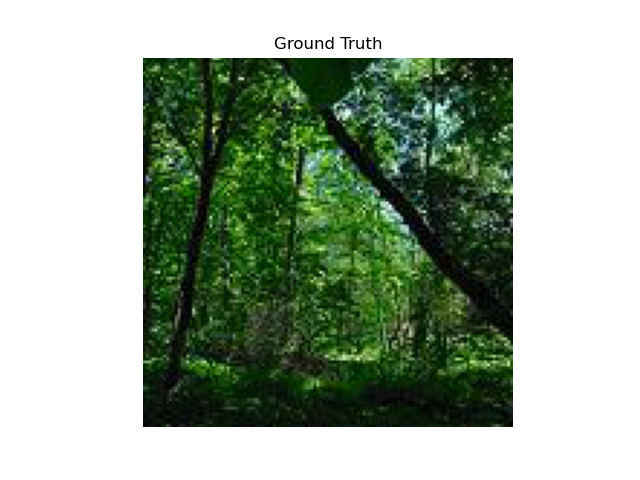
\includegraphics[width=.235\textwidth]{resources/experiments/landscape/324_bins/462/462_original.png}
  \end{subfigure}
  \begin{subfigure}
    \centering
    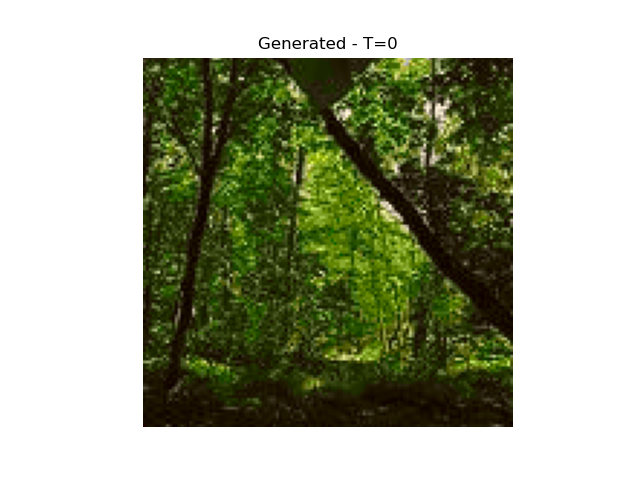
\includegraphics[width=.235\textwidth]{resources/experiments/landscape/324_bins/462/462_t0.png}
  \end{subfigure}
  \begin{subfigure}
    \centering
    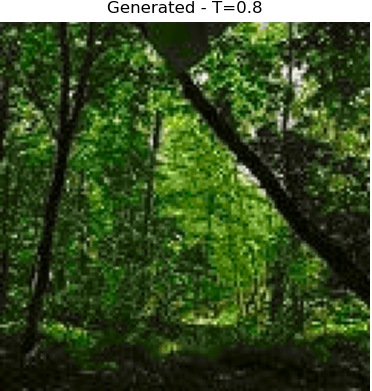
\includegraphics[width=.235\textwidth]{resources/experiments/landscape/324_bins/462/462_t08.png}
  \end{subfigure}
  \begin{subfigure}
    \centering
    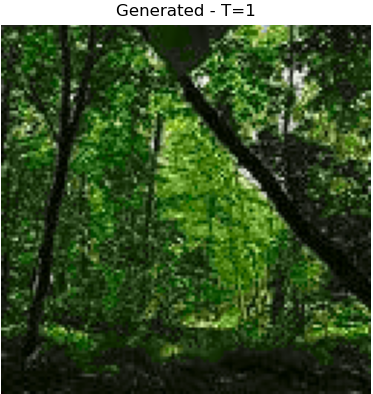
\includegraphics[width=.235\textwidth]{resources/experiments/landscape/324_bins/462/462_t1.png}
  \end{subfigure}

  \begin{subfigure}
    \centering
    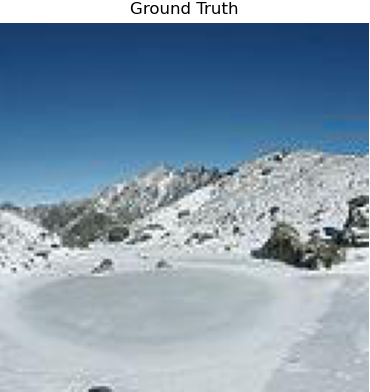
\includegraphics[width=.235\textwidth]{resources/experiments/landscape/324_bins/716/716_original.png}
  \end{subfigure}
  \begin{subfigure}
    \centering
    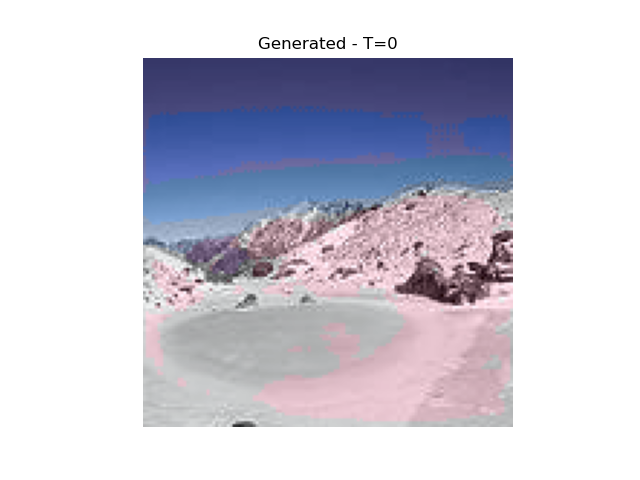
\includegraphics[width=.235\textwidth]{resources/experiments/landscape/324_bins/716/716_t0.png}
  \end{subfigure}
  \begin{subfigure}
    \centering
    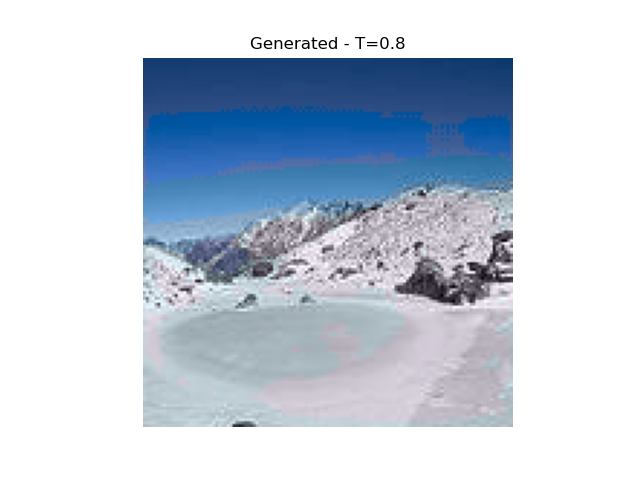
\includegraphics[width=.235\textwidth]{resources/experiments/landscape/324_bins/716/716_t08.png}
  \end{subfigure}
  \begin{subfigure}
    \centering
    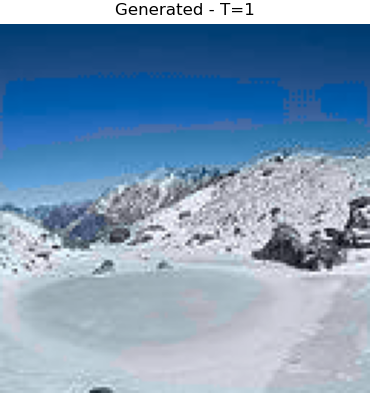
\includegraphics[width=.235\textwidth]{resources/experiments/landscape/324_bins/716/716_t1.png}
  \end{subfigure}
  
  \caption{Ergebnisse mit 324 Bins. Die erste Spalte zeigt das Originale Bild, die zweite zeigt das generierte Bild mit einer Temperatur von 0,
  die dritte Spalte zeigt das generierte Bild mit einer Temperatur von 0.8 und die vierte Spalte zeigt das generierte Bild mit einer Temperatur 
  von 1}
\end{figure}

\begin{figure}[H]
  \begin{subfigure}
    \centering
    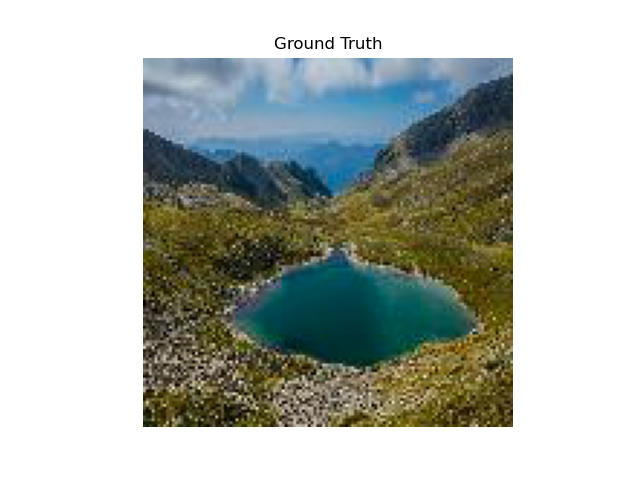
\includegraphics[width=.235\textwidth]{resources/experiments/landscape/324_bins/2414/2414_original.png}
  \end{subfigure}
  \begin{subfigure}
    \centering
    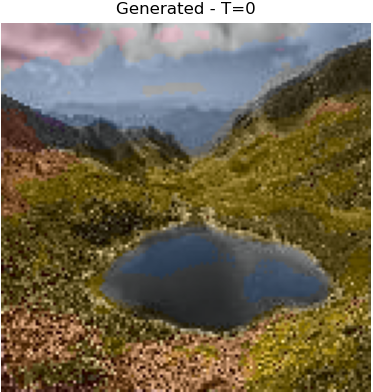
\includegraphics[width=.235\textwidth]{resources/experiments/landscape/324_bins/2414/2414_t0.png}
  \end{subfigure}
  \begin{subfigure}
    \centering
    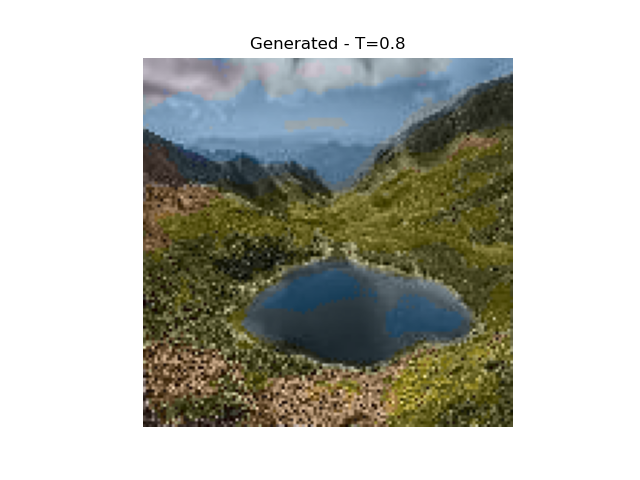
\includegraphics[width=.235\textwidth]{resources/experiments/landscape/324_bins/2414/2414_t08.png}
  \end{subfigure}
  \begin{subfigure}
    \centering
    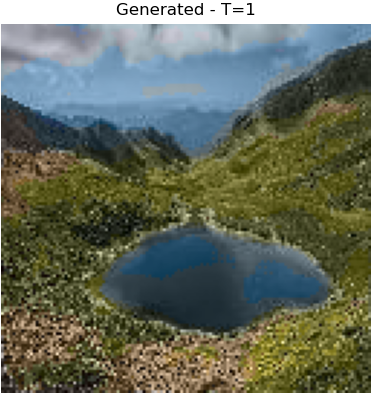
\includegraphics[width=.235\textwidth]{resources/experiments/landscape/324_bins/2414/2414_t1.png}
  \end{subfigure}

  \begin{subfigure}
    \centering
    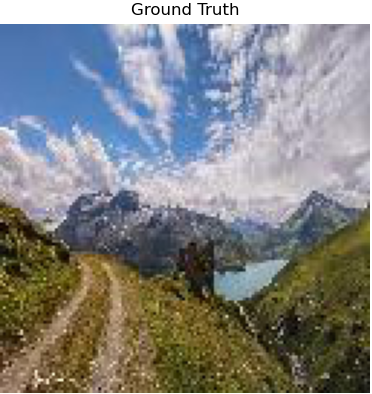
\includegraphics[width=.235\textwidth]{resources/experiments/landscape/324_bins/2441/2441_original.png}
  \end{subfigure}
  \begin{subfigure}
    \centering
    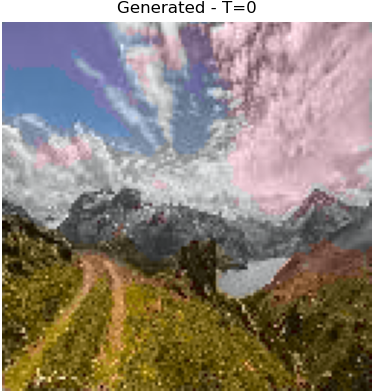
\includegraphics[width=.235\textwidth]{resources/experiments/landscape/324_bins/2441/2441_t0.png}
  \end{subfigure}
  \begin{subfigure}
    \centering
    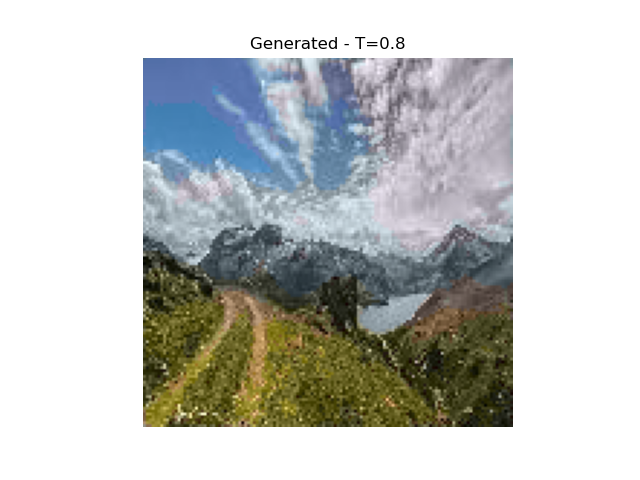
\includegraphics[width=.235\textwidth]{resources/experiments/landscape/324_bins/2441/2441_t08.png}
  \end{subfigure}
  \begin{subfigure}
    \centering
    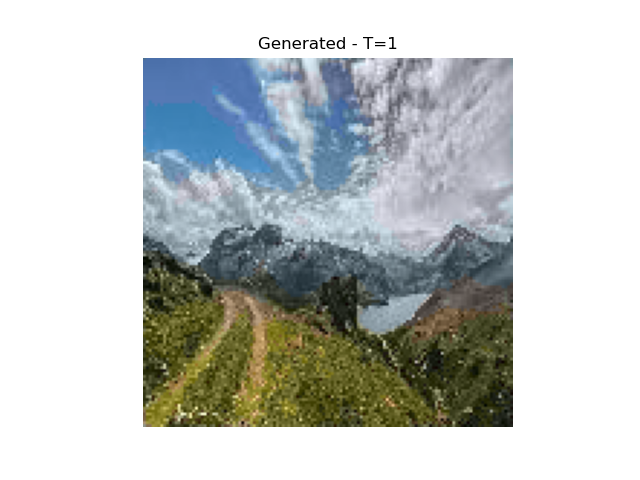
\includegraphics[width=.235\textwidth]{resources/experiments/landscape/324_bins/2441/2441_t1.png}
  \end{subfigure}

  \begin{subfigure}
    \centering
    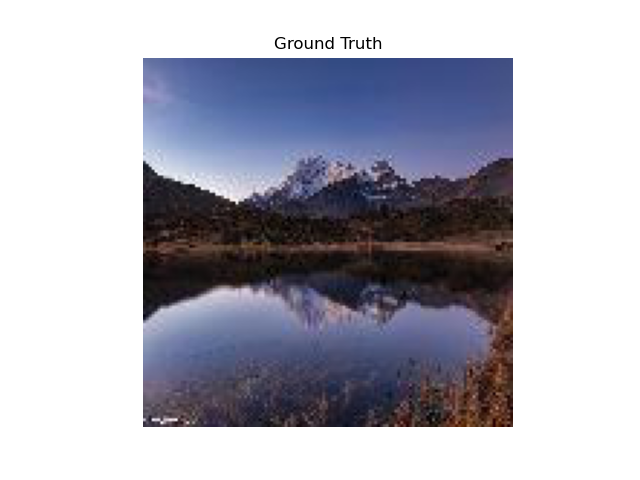
\includegraphics[width=.235\textwidth]{resources/experiments/landscape/324_bins/2512/2512_original.png}
  \end{subfigure}
  \begin{subfigure}
    \centering
    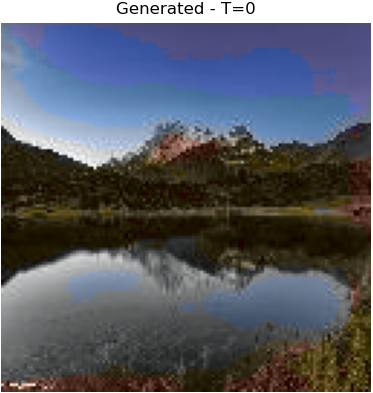
\includegraphics[width=.235\textwidth]{resources/experiments/landscape/324_bins/2512/2512_t0.png}
  \end{subfigure}
  \begin{subfigure}
    \centering
    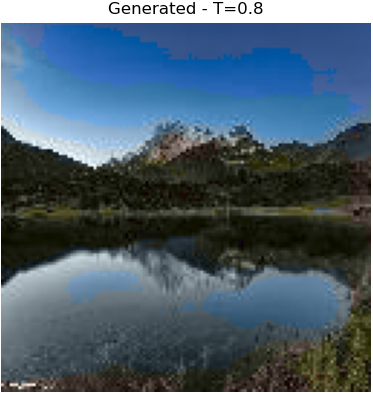
\includegraphics[width=.235\textwidth]{resources/experiments/landscape/324_bins/2512/2512_t08.png}
  \end{subfigure}
  \begin{subfigure}
    \centering
    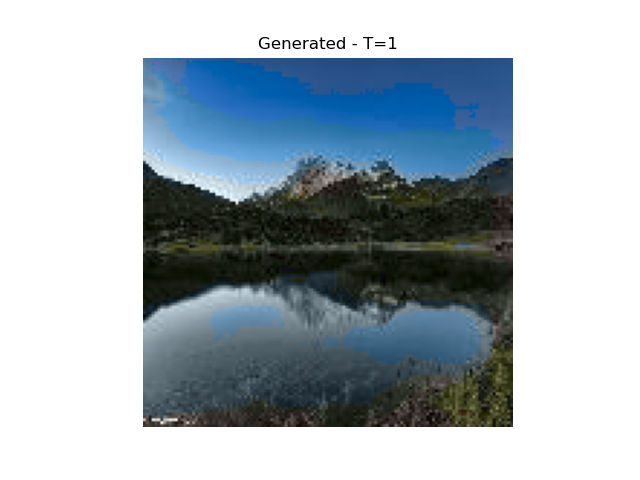
\includegraphics[width=.235\textwidth]{resources/experiments/landscape/324_bins/2512/2512_t1.png}
  \end{subfigure}

  \begin{subfigure}
    \centering
    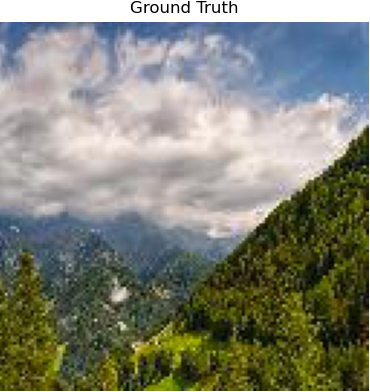
\includegraphics[width=.235\textwidth]{resources/experiments/landscape/324_bins/2615/2615_original.png}
  \end{subfigure}
  \begin{subfigure}
    \centering
    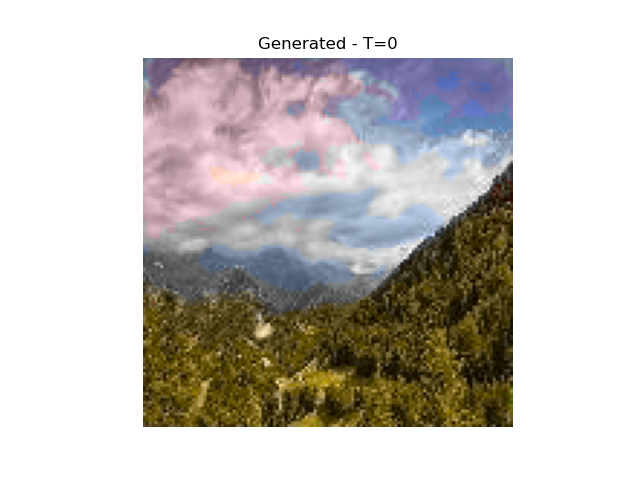
\includegraphics[width=.235\textwidth]{resources/experiments/landscape/324_bins/2615/2615_t0.png}
  \end{subfigure}
  \begin{subfigure}
    \centering
    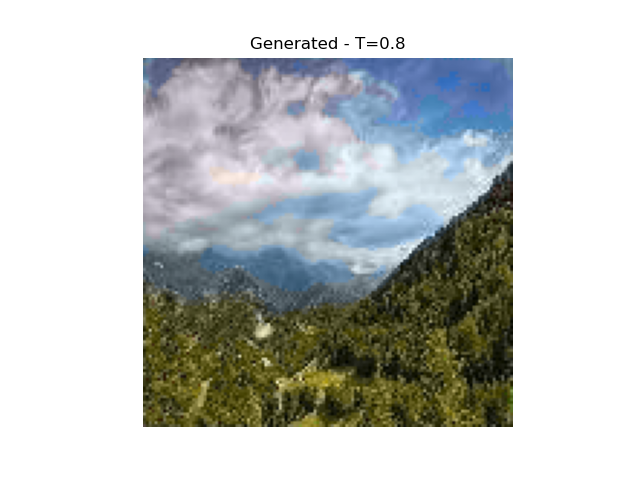
\includegraphics[width=.235\textwidth]{resources/experiments/landscape/324_bins/2615/2615_t08.png}
  \end{subfigure}
  \begin{subfigure}
    \centering
    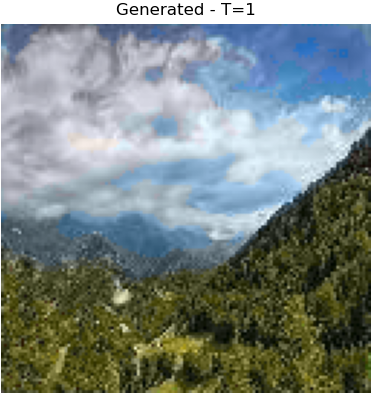
\includegraphics[width=.235\textwidth]{resources/experiments/landscape/324_bins/2615/2615_t1.png}
  \end{subfigure}

  \begin{subfigure}
    \centering
    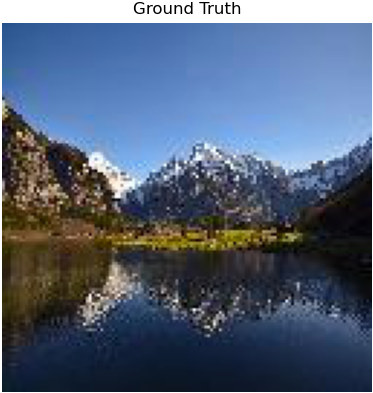
\includegraphics[width=.235\textwidth]{resources/experiments/landscape/324_bins/2639/2639_original.png}
  \end{subfigure}
  \begin{subfigure}
    \centering
    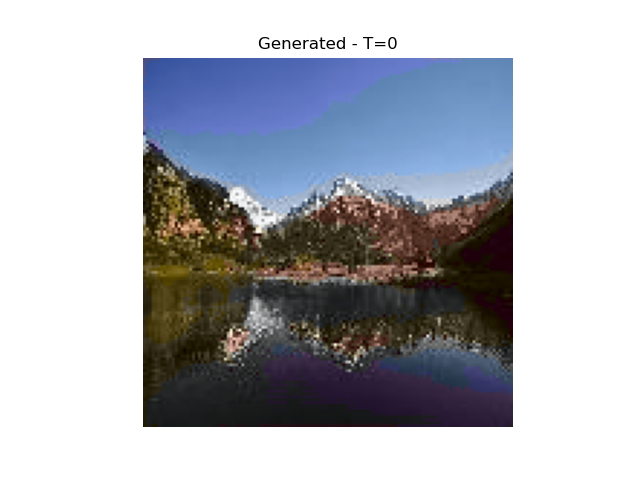
\includegraphics[width=.235\textwidth]{resources/experiments/landscape/324_bins/2639/2639_t0.png}
  \end{subfigure}
  \begin{subfigure}
    \centering
    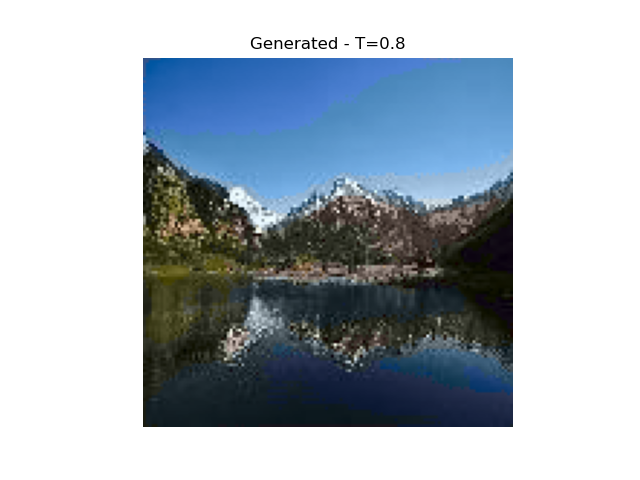
\includegraphics[width=.235\textwidth]{resources/experiments/landscape/324_bins/2639/2639_t08.png}
  \end{subfigure}
  \begin{subfigure}
    \centering
    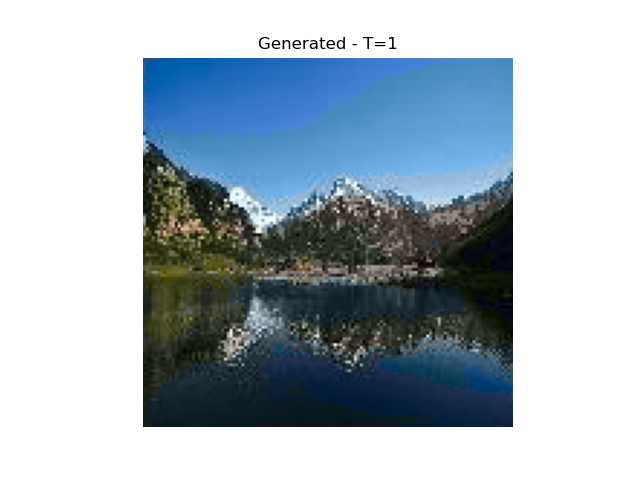
\includegraphics[width=.235\textwidth]{resources/experiments/landscape/324_bins/2639/2639_t1.png}
  \end{subfigure}

  \caption{Ergebnisse mit 324 Bins. Die erste Spalte zeigt das Originale Bild, die zweite zeigt das generierte Bild mit einer Temperatur von 0,
  die dritte Spalte zeigt das generierte Bild mit einer Temperatur von 0.8 und die vierte Spalte zeigt das generierte Bild mit einer Temperatur 
  von 1}
\end{figure}

\begin{figure}[H]
  \begin{subfigure}
    \centering
    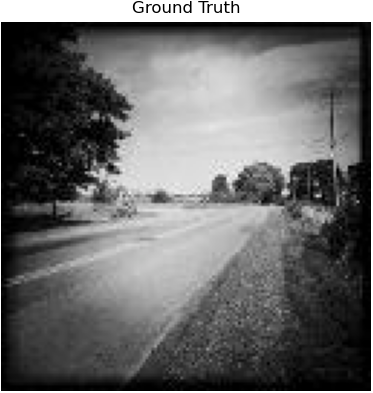
\includegraphics[width=.235\textwidth]{resources/experiments/landscape/324_bins/1750/1750_original.png}
  \end{subfigure}
  \begin{subfigure}
    \centering
    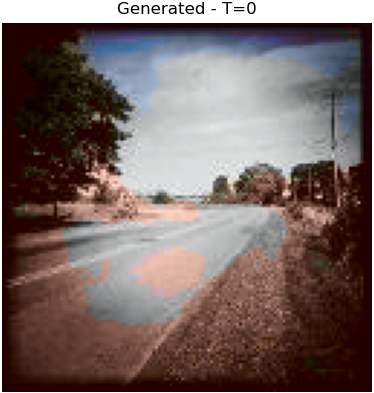
\includegraphics[width=.235\textwidth]{resources/experiments/landscape/324_bins/1750/1750_t0.png}
  \end{subfigure}
  \begin{subfigure}
    \centering
    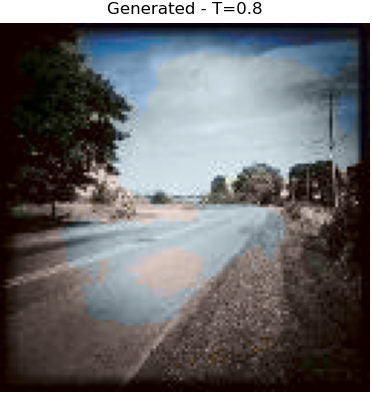
\includegraphics[width=.235\textwidth]{resources/experiments/landscape/324_bins/1750/1750_t08.png}
  \end{subfigure}
  \begin{subfigure}
    \centering
    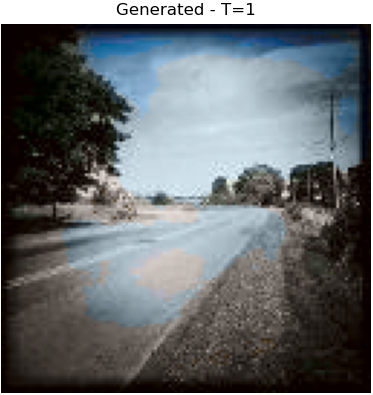
\includegraphics[width=.235\textwidth]{resources/experiments/landscape/324_bins/1750/1750_t1.png}
  \end{subfigure}

  \begin{subfigure}
    \centering
    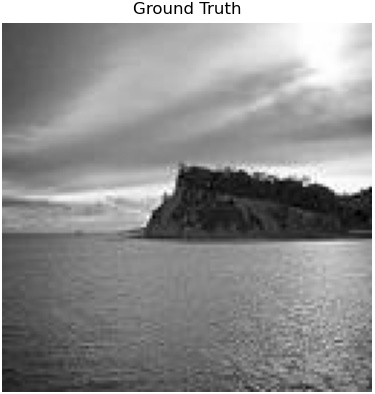
\includegraphics[width=.235\textwidth]{resources/experiments/landscape/324_bins/1915/1915_original.png}
  \end{subfigure}
  \begin{subfigure}
    \centering
    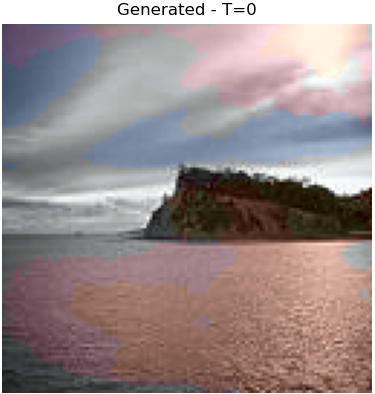
\includegraphics[width=.235\textwidth]{resources/experiments/landscape/324_bins/1915/1915_t0.png}
  \end{subfigure}
  \begin{subfigure}
    \centering
    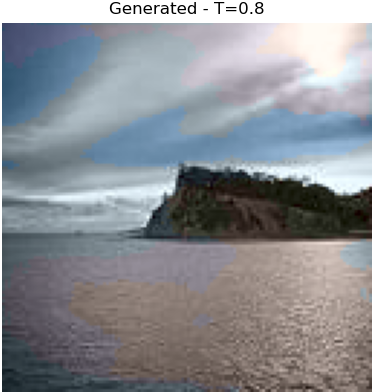
\includegraphics[width=.235\textwidth]{resources/experiments/landscape/324_bins/1915/1915_t08.png}
  \end{subfigure}
  \begin{subfigure}
    \centering
    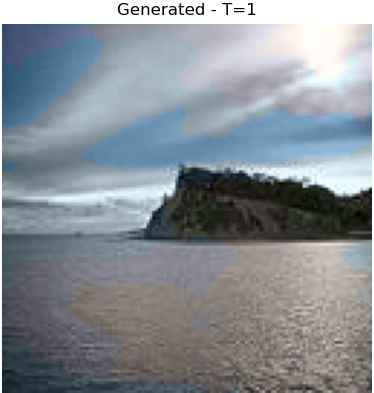
\includegraphics[width=.235\textwidth]{resources/experiments/landscape/324_bins/1915/1915_t1.png}
  \end{subfigure}

  \caption{Ergebnisse mit 324 Bins wo das Original Bild ein Graustufenbild ist.}
\end{figure}

\section{Notebook CIFAR-100 Subset Colorization}
\label{sec:nootebook_cifar_100}
\begin{longlisting}
  \begin{minted}{python}
    from __future__ import print_function, division
    import time
    import datetime
    import os
    import copy
    import csv

    import matplotlib.pyplot as plt

    # For conversion
    from skimage.color import lab2rgb, rgb2lab, rgb2gray
    from skimage import io

    import numpy as np
    import torch
    import torch.utils.data
    import torch.nn as nn
    import torch.nn.functional as F
    import torch.optim as optim
    from torch.optim import lr_scheduler
    from torch.optim.lr_scheduler import ReduceLROnPlateau
    import torchvision
    from torchvision import datasets, models, transforms

    use_gpu = torch.cuda.is_available()
    N_BINS = 324
    W_BIN  = np.sqrt(N_BINS).astype(int)

    cifar_data_train = datasets.CIFAR100(".", train=True, transform=transforms.Compose([
      transforms.RandomResizedCrop(32),
      transforms.RandomHorizontalFlip()
    ]), target_transform=None, download=True)

    cifar_data_val = datasets.CIFAR100(".", train=False, transform=transforms.Compose([
      transforms.Resize(32),
      transforms.CenterCrop(32)
    ]), target_transform=None, download=True)

    meta = np.load('cifar-100-python/meta', allow_pickle=True)

    def calculate_bin(a, b, width):
      return (width * b) + a

    '''
      Encode each pixel from the image into a bin

      Output: (W, H) where each value is a bin
    '''
    def encode_bins(ab_image, n_bins):
      x = np.linspace(0,1,W_BIN+1)
      indices = np.digitize(ab_image, x) - 1
      
      bins = np.vectorize(calculate_bin)(indices[:,:,0], indices[:,:,1], W_BIN)

      return bins

    def to_rgb(grayscale_input, ab_input):
      '''
        Convert to rgb
      '''
      color_image = torch.cat((grayscale_input, ab_input), 0).numpy() #combine channels
      color_image = color_image.transpose((1, 2, 0)) # rescale for matplotlib
      color_image[:, :, 0:1] = color_image[:, :, 0:1] * 100
      color_image[:, :, 1:3] = color_image[:, :, 1:3] * 255 - 128
      color_image = lab2rgb(color_image)
      
      return (color_image * 255).astype(int)

    class GrayscaleDataLoader(torch.utils.data.Dataset):
      def __init__(self, dataset):
        self.images = dataset

      def __getitem__(self, index):
        image, target = self.images[index]
        
        img_original = np.asarray(image)

        # rgb to lab
        img_lab = rgb2lab(img_original)
        img_lab = (img_lab + 128) / 255
        img_ab = img_lab[:, :, 1:3]

        # form bins
        bins = torch.from_numpy(encode_bins(img_ab, N_BINS))

        #ab channels
        img_ab = torch.from_numpy(img_ab.transpose((2, 0, 1))).float()

        # greyscale image
        img_original = rgb2gray(img_original)
        img_original = torch.from_numpy(img_original).unsqueeze(0).float()
        
        return img_original, img_ab, bins

      def __len__(self):
        return len(self.images)

    classes = [0, 23, 33, 47, 49, 52, 56, 59, 70, 71, 82, 96]

    def filter_image(image):
      if image[1] in classes:
        return image

    filtered_data_train = list(filter(None, map(filter_image, cifar_data_train)))
    train_images = GrayscaleDataLoader(cifar_data_train)

    filtered_data_val = list(filter(None, map(filter_image, cifar_data_val)))
    val_images = GrayscaleDataLoader(cifar_data_val)

    print(len(train_images))
    print(len(val_images))

    train_loader = torch.utils.data.DataLoader(train_images, batch_size=64, shuffle=True)
    val_loader = torch.utils.data.DataLoader(val_images, batch_size=64, shuffle=True)

    class Conv2dBlock(nn.Module):
      def __init__(self, D_in, n_filters, kernel_size=3):
        super(Conv2dBlock, self).__init__()

        # first layer
        self.conv1       = nn.Conv2d(D_in, n_filters, kernel_size, stride=1, padding=1)
        self.batch_norm1 = nn.BatchNorm2d(n_filters)

        # second layer
        self.conv2       = nn.Conv2d(n_filters, n_filters, kernel_size, stride=1, padding=1)
        self.batch_norm2 = nn.BatchNorm2d(n_filters)
      
      def forward(self, x):
        x = self.conv1(x)
        x = self.batch_norm1(x)
        x = F.relu(x)
        x = self.conv2(x)
        x = self.batch_norm2(x)
        out = F.relu(x)
      
        return out

    class Model(nn.Module):
      def __init__(self, n_out):
        super(Model, self).__init__()
        
        # Encoder
        self.conv1 = Conv2dBlock(1, 8)
        self.pool1 = nn.MaxPool2d(2, 2)

        self.conv2 = Conv2dBlock(8, 16)
        self.pool2 = nn.MaxPool2d(2, 2)

        self.conv3 = Conv2dBlock(16, 32)

        # Decoder
        self.upconv1 = nn.ConvTranspose2d(32, 16, kernel_size=3, stride=2, padding=1, output_padding=1)

        self.conv4   = Conv2dBlock(32, 16)
        self.upconv2 = nn.ConvTranspose2d(16, 8, kernel_size=3, stride=2, padding=1, output_padding=1)

        self.conv5   = Conv2dBlock(16, 8)
        self.conv6   = nn.Conv2d(8, n_out, kernel_size=1, stride=1, padding=0)
        
      def forward(self, x):
        c1 = self.conv1(x)
        x  = self.pool1(c1)

        c2 = self.conv2(x)
        x  = self.pool2(c2)

        c3 = self.conv3(x)

        u1 = self.upconv1(c3)
        x  = torch.cat([u1, c2], dim=1)

        x = self.conv4(x)
        u2 = self.upconv2(x)
        x  = torch.cat([u2, c1], dim=1)

        x = self.conv5(x)
        out = self.conv6(x)

        return out

    # Classify mode colors to bins
    dataset_bin_colors = {i: [[], []] for i in range(N_BINS)}

    def get_dataset_bin(colors_dict, mode='mode'):
      _dict = copy.deepcopy(colors_dict)

      for bin in _dict:
        for channel, _ in enumerate(_dict[bin]):
          if (len(_dict[bin][channel]) > 0):
            if mode == 'mode':
              _dict[bin][channel] = np.max(np.array(_dict[bin][channel]))
            elif mode == 'mean':
              _dict[bin][channel] = np.mean(np.array(_dict[bin][channel]))
          else:
            _dict[bin][channel] = 0

      np.save(mode + '_color_bins_'+str(N_BINS)+'.npy', _dict)
      del _dict

    def add_to_dict(bin, a, b):
      dataset_bin_colors[bin][0].append(a)
      dataset_bin_colors[bin][1].append(b)

    def _encode_bins(ab_image):
      x = np.linspace(0,1,W_BIN+1)
      indices = np.digitize(ab_image, x) - 1
      indices = indices.transpose(1, 2, 0)
      
      bins = np.vectorize(calculate_bin)(indices[:,:,0], indices[:,:,1], W_BIN)
      np.vectorize(add_to_dict)(bins, ab_image[0,:,:], ab_image[1,:,:])

      return bins

    counter = 0

    for index, y in enumerate(train_loader):
      gray_images, ab_images, bins = y
        
      for i, ab in enumerate(ab_images):
        _encode_bins(ab)

    get_dataset_bin(dataset_bin_colors, 'mode')
    get_dataset_bin(dataset_bin_colors, 'mean')

    '''
      Return the mode of the predicted bin for each color chanel
    '''
    def decode_pixel(bin, T, dataset_bin_colors_mode, dataset_bin_colors_mean):
      a_mode = dataset_bin_colors_mode[bin][0]
      b_mode = dataset_bin_colors_mode[bin][1]

      a_mean = dataset_bin_colors_mean[bin][0]
      b_mean = dataset_bin_colors_mean[bin][1]

      if a_mode == 0:
        a_mode = assign_next_bin(bin, a_mode, 0, dataset_bin_colors_mode)

      if b_mode == 0:
        b_mode = assign_next_bin(bin, b_mode, 1, dataset_bin_colors_mode)

      if a_mean == 0:
        a_mean = assign_next_bin(bin, a_mean, 0, dataset_bin_colors_mean)

      if b_mean == 0:
        b_mean = assign_next_bin(bin, b_mean, 1, dataset_bin_colors_mean)
      
      a_distance = a_mode - a_mean
      b_distance = b_mode - b_mean

      a = a_mode - (a_distance * T)
      b = b_mode - (b_distance * T)

      return a, b

    '''
      Assign predicted color from next bin
    '''
    def assign_next_bin(bin, channel, index, colormap):
      counter = [1, -1]
      length = len(colormap) - 1

      while channel == 0:
        plus_index = bin + counter[0] if bin + counter[0] <= length else length
        channel = colormap[plus_index][index]

        if channel == 0:
          counter[0] += 1
          minus_index = bin + counter[1] if bin + counter[1] >= 0 else 0
          channel = colormap[minus_index][index]
          counter[1] -= 1

      return channel

    def deserialize_bins(bins, T, mode_path, mean_path):
      bins = bins.numpy()
      dataset_bin_colors_mode = np.load(mode_path, allow_pickle=True)
      dataset_bin_colors_mean = np.load(mean_path, allow_pickle=True)

      return np.array(np.vectorize(decode_pixel)(bins, T, dataset_bin_colors_mode, dataset_bin_colors_mean))

    '''
      A class from the PyTorch ImageNet tutorial
    ''' 
    class AverageMeter(object):
      def __init__(self):
        self.reset()
      def reset(self):
        self.val, self.avg, self.sum, self.count = 0, 0, 0, 0
      def update(self, val, n=1):
        self.val = val
        self.sum += val * n
        self.count += n
        self.avg = self.sum / self.count

    def train(train_loader, model, criterion, optimizer, epoch, use_gpu):
      print('Starting training epoch {}'.format(epoch))
      model.train()

      # Prepare value counters and timers
      batch_time, data_time, losses = AverageMeter(), AverageMeter(), AverageMeter()

      end = time.time()
      for i, (input_gray, input_ab, bins) in enumerate(train_loader):
        bins = bins.squeeze(0)
        # Use GPU if available
        if use_gpu: input_gray, input_ab, bins = input_gray.cuda(), input_ab.cuda(), bins.cuda()

        # Record time to load data (above)
        data_time.update(time.time() - end)

        # Run forward pass
        output_bins = model(input_gray)
        loss = criterion(output_bins, bins)
        losses.update(loss.item(), input_gray.size(0))

        # Compute gradient and optimize
        optimizer.zero_grad()
        loss.backward()
        optimizer.step()

        # Record time to do forward and backward passes
        batch_time.update(time.time() - end)
        end = time.time()

        # Print model accuracy -- in the code below, val refers to value, not validation
        if i % 25 == 0:
          print('Epoch: [{0}][{1}/{2}]\t'
                'Time {batch_time.val:.3f} ({batch_time.avg:.3f})\t'
                'Data {data_time.val:.3f} ({data_time.avg:.3f})\t'
                'Loss {loss.val:.4f} ({loss.avg:.4f})\t'.format(
                  epoch, i, len(train_loader), batch_time=batch_time,
                data_time=data_time, loss=losses))

      print('Finished training epoch {}'.format(epoch))

      return losses.avg

    def validate(val_loader, model, criterion, epoch, use_gpu):
      model.eval()

      # Prepare value counters and timers
      batch_time, data_time, losses = AverageMeter(), AverageMeter(), AverageMeter()

      end = time.time()

      for i, (input_gray, input_ab, bins) in enumerate(val_loader):
        data_time.update(time.time() - end)
        bins = bins.squeeze(0)

        # Use GPU
        if use_gpu: input_gray, input_ab, bins = input_gray.cuda(), input_ab.cuda(), bins.cuda()

        # Run model and record loss
        output_bins = model(input_gray)
        loss = criterion(output_bins, bins)
        losses.update(loss.item(), input_gray.size(0))

        # Record time to do forward passes and save images
        batch_time.update(time.time() - end)
        end = time.time()

        # Print model accuracy -- in the code below, val refers to both value and validation
        if i % 25 == 0:
          print('Validate: [{0}/{1}]\t'
                'Time {batch_time.val:.3f} ({batch_time.avg:.3f})\t'
                'Loss {loss.val:.4f} ({loss.avg:.4f})\t'.format(i, len(val_loader), batch_time=batch_time, loss=losses))

      print('Finished validation.')
      return losses.avg

    model = Model(324)
    criterion = nn.CrossEntropyLoss()
    optimizer = torch.optim.Adam(model.parameters(), lr=0.001)

    if use_gpu:
      criterion = criterion.cuda()
      model = model.cuda()

    epochs = 150
    best_losses = 2.5

    output = csv.writer(open('train_log.csv', 'w'))
    output.writerow(['epoch', 'train_loss', 'val_loss'])

    with open('train_log.csv', 'w') as output:
      writer = csv.writer(output)
      writer.writerow(['epoch', 'train_loss', 'val_loss'])

      for epoch in range(60, epochs):
        if use_gpu and epoch > 0:
          model.cuda()
        # Train for one epoch, then validate
        train_loss = train(train_loader, model, criterion, optimizer, epoch, use_gpu)
        with torch.no_grad():
          val_loss = validate(val_loader, model, criterion, epoch, use_gpu)
          # scheduler.step(val_loss)
        writer.writerow([epoch, train_loss, val_loss])
        # Save checkpoint and replace old best model if current model is better
        print('Val Loss = {}'.format(val_loss))
        print('Best Loss = {}'.format(best_losses))
        if val_loss < best_losses:
          best_losses = val_loss
          torch.save(model.to('cpu').state_dict(), 'model-cifar-{}-{}-{:.3f}.pth'.format(N_BINS, epoch+1,val_loss))

    def evaluate(gray, ab_input, bins, model, temperature):
      model.eval()

      with torch.no_grad():
        bins = bins.squeeze(0)

        # Run model and record loss
        # add batch size 1 for single image
        output_bins = model(gray.unsqueeze(1))
        
        # remove batch size and get the max index of the predicted bin for each pixel
        color_image = to_rgb(
          gray,
          torch.from_numpy(
            deserialize_bins(
              output_bins.squeeze(0).argmax(0),
              temperature,
              'mode_color_bins_'+str(N_BINS)+'.npy',
              'mean_color_bins_'+str(N_BINS)+'.npy',
            ),
          ).float()
        )

      return color_image
  \end{minted}
\end{longlisting}

\section{Skripte Lanscape Datensatz Colorization}
\subsection{Image augmentation Skript}
\begin{longlisting}
  \begin{minted}{python}
    import os
    from glob import glob

    import imageio
    import imgaug as ia
    import imgaug.augmenters as iaa
    import numpy as np
    import pandas as pd
    import matplotlib.pyplot as plt
    import matplotlib.patches as patches
    import matplotlib

    DATASET_PATH = "dataset_clean/train/"
    DATASET_VAL_PATH = "dataset_clean/val/"
    AUGUMENTED_PATH = "dataset_resized/train/"
    AUGUMENTED_VAL_PATH = "dataset_resized/val/"
    CLASSES = ["field", "forest", "glacier", "lake", "mountain", "road", "sea", "uncategorized"]
    SIZE = 128

    for _class in CLASSES:
      train_files = glob("./{}{}/*".format(AUGUMENTED_PATH, _class))
      val_files = glob("./{}{}/*".format(AUGUMENTED_VAL_PATH, _class))

      for f in train_files:
        os.remove(f)

      for f in val_files:
        os.remove(f)

    aug = iaa.Resize({"height": SIZE, "width": SIZE}, "cubic")
    rotate=iaa.Affine(rotate=(-30, 30))
    crop = iaa.Crop(percent=(0, 0.3))
    flip_hr=iaa.Fliplr(p=1.0)
    flip_vr=iaa.Flipud(p=1.0)

    # Resize training images to the given size
    for i, _class in enumerate(CLASSES):
      for filename in os.listdir(DATASET_PATH + "/" + CLASSES[i]):
        image = imageio.imread(DATASET_PATH + "/" + CLASSES[i] + "/" + filename)
        augumented_img = aug.augment_image(image)
        imageio.imwrite(AUGUMENTED_PATH + "/" + CLASSES[i] + "/" + filename, augumented_img)

    # Resize validation images to the given size
    for i, _class in enumerate(CLASSES):
      for filename in os.listdir(DATASET_VAL_PATH + "/" + CLASSES[i]):
        image = imageio.imread(DATASET_VAL_PATH + "/" + CLASSES[i] + "/" + filename)
        augumented_img = aug.augment_image(image)
        imageio.imwrite(AUGUMENTED_VAL_PATH + "/" + CLASSES[i] + "/" + filename, augumented_img)

    # Apply argumentation to the images
    for i, _class in enumerate(CLASSES):
      for filename in os.listdir(AUGUMENTED_PATH + "/" + CLASSES[i]):
        image = imageio.imread(AUGUMENTED_PATH + "/" + CLASSES[i] + "/" + filename)

        # Rotate image between -30 and 30 degrees
        rotated_image=rotate.augment_image(image)
        imageio.imwrite(AUGUMENTED_PATH + "/" + CLASSES[i] + "/rotated_" + filename, rotated_image)

        # Crop image by a factor of 30%
        cropped_image=crop.augment_image(image)
        imageio.imwrite(AUGUMENTED_PATH + "/" + CLASSES[i] + "/croped_" + filename, cropped_image)

        # Flip image horizontaly
        flip_hr_image= flip_hr.augment_image(image)
        imageio.imwrite(AUGUMENTED_PATH + "/" + CLASSES[i] + "/hr_flipped_" + filename, flip_hr_image)

        # Flip image verticaly
        flip_vr_image= flip_vr.augment_image(image)
        imageio.imwrite(AUGUMENTED_PATH + "/" + CLASSES[i] + "/vr_flipped_" + filename, flip_vr_image)

  \end{minted}
\end{longlisting}

\subsection{Modell Skript}
\begin{longlisting}
  \begin{minted}{python}
    from __future__ import print_function, division

    import numpy as np
    import torch
    import torch.nn as nn
    import torch.nn.functional as F

    class Conv2dBlock(nn.Module):
      def __init__(self, D_in, n_filters, kernel_size=3):
        super(Conv2dBlock, self).__init__()

        # first layer
        self.conv1       = nn.Conv2d(D_in, n_filters, kernel_size, stride=1, padding=1)
        self.batch_norm1 = nn.BatchNorm2d(n_filters)

        # second layer
        self.conv2       = nn.Conv2d(n_filters, n_filters, kernel_size, stride=1, padding=1)
        self.batch_norm2 = nn.BatchNorm2d(n_filters)
      
      def forward(self, x):
        x = self.conv1(x)
        x = self.batch_norm1(x)
        x = F.relu(x)
        x = self.conv2(x)
        x = self.batch_norm2(x)
        out = F.relu(x)

        return out

    class Model(nn.Module):
      def __init__(self, n_out, divider=1):
        super(Model, self).__init__()
        
        # Encoder
        self.conv1 = Conv2dBlock(1, int(16 / divider))
        self.pool1 = nn.MaxPool2d(2, 2)

        self.conv2 = Conv2dBlock(int(16 / divider), int(32 / divider))
        self.pool2 = nn.MaxPool2d(2, 2)

        self.conv3 = Conv2dBlock(int(32 / divider), int(64 / divider))
        self.pool3 = nn.MaxPool2d(2, 2)

        self.conv4 = Conv2dBlock(int(64 / divider), int(128 / divider))
        self.pool4 = nn.MaxPool2d(2, 2)

        self.conv5 = Conv2dBlock(int(128 / divider), int(256 / divider))

        # Decoder
        self.upconv6 = nn.ConvTranspose2d(int(256 / divider), int(128 / divider), kernel_size=3, stride=2, padding=1, output_padding=1)

        self.conv6   = Conv2dBlock(int(256 / divider), int(128 / divider))
        self.upconv7 = nn.ConvTranspose2d(int(128 / divider), int(64 / divider), kernel_size=3, stride=2, padding=1, output_padding=1)

        self.conv7   = Conv2dBlock(int(128 / divider), int(64 / divider))
        self.upconv8 = nn.ConvTranspose2d(int(64 / divider), int(32 / divider), kernel_size=3, stride=2, padding=1, output_padding=1)

        self.conv8   = Conv2dBlock(int(64 / divider), int(32 / divider))
        self.upconv9 = nn.ConvTranspose2d(int(32 / divider), int(16 / divider), kernel_size=3, stride=2, padding=1, output_padding=1)

        self.conv9   = Conv2dBlock(int(32 / divider), int(16 / divider))
        self.conv10   = nn.Conv2d(int(16 / divider), n_out, kernel_size=1, stride=1, padding=0)

      def forward(self, x):
        c1 = self.conv1(x)
        x  = self.pool1(c1)

        c2 = self.conv2(x)
        x  = self.pool2(c2)

        c3 = self.conv3(x)
        x  = self.pool3(c3)

        c4 = self.conv4(x)
        x  = self.pool4(c4)

        c5 = self.conv5(x)

        u6 = self.upconv6(c5)
        x  = torch.cat([u6, c4], dim=1)

        x = self.conv6(x)

        u7 = self.upconv7(x)
        x  = torch.cat([u7, c3], dim=1)

        x = self.conv7(x)

        u8 = self.upconv8(x)
        x  = torch.cat([u8, c2], dim=1)

        x  = self.conv8(x)

        u9 = self.upconv9(x)
        x  = torch.cat([u9, c1], dim=1)

        x  = self.conv9(x)

        out = self.conv10(x)

        return out
  \end{minted}
\end{longlisting}

\subsection{Utils Skript}
\begin{longlisting}
  \begin{minted}{python}
    from __future__ import print_function, division
    import time
    import os
    import copy

    from skimage.color import lab2rgb, rgb2lab, rgb2gray
    from skimage import io

    import numpy as np
    import torch
    from torchvision import datasets, models, transforms

    class AverageMeter(object):
      '''A handy class from the PyTorch ImageNet tutorial''' 
      def __init__(self):
        self.reset()
      def reset(self):
        self.val, self.avg, self.sum, self.count = 0, 0, 0, 0
      def update(self, val, n=1):
        self.val = val
        self.sum += val * n
        self.count += n
        self.avg = self.sum / self.count

    def load_img(img, N_BINS):
      img_original = np.asarray(img)
      
      # rgb to lab
      img_lab = rgb2lab(img_original)
      img_lab = (img_lab + 128) / 255
      img_ab = img_lab[:, :, 1:3]

      
      # form bins
      bins = torch.from_numpy(encode_bins(img_ab, N_BINS))

      #ab channels
      img_ab = torch.from_numpy(img_ab.transpose((2, 0, 1))).float()
      
      # greyscale image
      img_original = rgb2gray(img_original)
      img_original = torch.from_numpy(img_original).unsqueeze(0).float()
      
      return img_original, img_ab, bins
        
    '''
      Generate a dictionary with the mode of every bin

      Output: BIN_NUMBER: [A_COLOR_MODE, B_COLOR_MODE] 
    '''
    def get_dataset_bin_mode(colors_dict):
      mode_dict = copy.deepcopy(colors_dict)

      for bin in mode_dict:
        for channel, _ in enumerate(mode_dict[bin]):
          if (len(mode_dict[bin][channel]) > 0):
            mode_dict[bin][channel] = np.max(np.array(mode_dict[bin][channel]))
          else:
            mode_dict[bin][channel] = 0

      return mode_dict

    '''
      Calculate the bin from the indices

      Output: N
    '''
    def calculate_bin(a, b, width):
      return (width * b) + a

    '''
      Add color to each bin dictionary value
    '''
    def add_to_dict(bin, a, b):
      dataset_bin_colors[bin][0].append(a)
      dataset_bin_colors[bin][1].append(b)


    '''
      Encode each pixel from the image into a bin

      Output: (W, H) where each value is a bin
    '''
    def encode_bins(ab_image, n_bins):
      w_bin  = np.sqrt(n_bins).astype(int)

      x = np.linspace(0,1,w_bin+1)
      indices = np.digitize(ab_image, x) - 1
      
      bins = np.vectorize(calculate_bin)(indices[:,:,0], indices[:,:,1], w_bin)

      return bins

    '''
      Return the mode of the predicted bin for each color chanel
    '''
    def decode_pixel(bin, T, dataset_bin_colors_mode, dataset_bin_colors_mean):
      a_mode = dataset_bin_colors_mode[bin][0]
      b_mode = dataset_bin_colors_mode[bin][1]

      a_mean = dataset_bin_colors_mean[bin][0]
      b_mean = dataset_bin_colors_mean[bin][1]

      if a_mode == 0:
        a_mode = assign_next_bin(bin, a_mode, 0, dataset_bin_colors_mode)

      if b_mode == 0:
        b_mode = assign_next_bin(bin, b_mode, 1, dataset_bin_colors_mode)

      if a_mean == 0:
        a_mean = assign_next_bin(bin, a_mean, 0, dataset_bin_colors_mean)

      if b_mean == 0:
        b_mean = assign_next_bin(bin, b_mean, 1, dataset_bin_colors_mean)
      
      a_distance = a_mode - a_mean
      b_distance = b_mode - b_mean

      a = a_mode - (a_distance * T)
      b = b_mode - (b_distance * T)

      return a, b

    '''
      Assign predicted color from next bin
    '''
    def assign_next_bin(bin, channel, index, colormap):
      counter = [1, -1]
      length = len(colormap) - 1

      while channel == 0:
        plus_index = bin + counter[0] if bin + counter[0] <= length else length
        channel = colormap[plus_index][index]

        if channel == 0:
          counter[0] += 1
          minus_index = bin + counter[1] if bin + counter[1] >= 0 else 0
          channel = colormap[minus_index][index]
          counter[1] -= 1

      return channel

    def serialize_bins(ab_image):
      return encode_bins(ab_image)

    def deserialize_bins(bins, T, mode_path, mean_path):
      bins = bins.numpy()
      dataset_bin_colors_mode = np.load(mode_path, allow_pickle=True)
      dataset_bin_colors_mean = np.load(mean_path, allow_pickle=True)

      return np.array(np.vectorize(decode_pixel)(bins, T, dataset_bin_colors_mode, dataset_bin_colors_mean))

    def to_rgb(grayscale_input, ab_input):
      '''
        Convert to rgb
      '''
      color_image = torch.cat((grayscale_input, ab_input), 0).numpy() #combine channels
      color_image = color_image.transpose((1, 2, 0)) # rescale for matplotlib
      color_image[:, :, 0:1] = color_image[:, :, 0:1] * 100
      color_image[:, :, 1:3] = color_image[:, :, 1:3] * 255 - 128
      color_image = lab2rgb(color_image)
      
      return (color_image * 255).astype(int)
  \end{minted}
\end{longlisting}

\subsection{Train Skript}
\begin{longlisting}
  \begin{minted}{python}
    import time
    from utils import AverageMeter

    def train(train_loader, model, criterion, optimizer, epoch, use_gpu=False):
      print('Starting training epoch {}'.format(epoch))
      model.train()

      # Prepare value counters and timers
      batch_time, data_time, losses = AverageMeter(), AverageMeter(), AverageMeter()

      end = time.time()
      for i, (input_gray, input_ab, bins) in enumerate(train_loader):
        bins = bins.squeeze(0)
        # Use GPU if available
        if use_gpu: input_gray, input_ab, bins = input_gray.cuda(), input_ab.cuda(), bins.cuda()

        # Record time to load data (above)
        data_time.update(time.time() - end)

        # Run forward pass
        output_bins = model(input_gray)

        if len(output_bins) != len(bins):
          bins = bins.unsqueeze(0)
        
        loss = criterion(output_bins, bins)
        losses.update(loss.item(), input_gray.size(0))

        # Compute gradient and optimize
        optimizer.zero_grad()
        loss.backward()
        optimizer.step()

        # Record time to do forward and backward passes
        batch_time.update(time.time() - end)
        end = time.time()

        # Print model accuracy -- in the code below, val refers to value, not validation
        if i % 25 == 0:
          print('Epoch: [{0}][{1}/{2}]\t'
                'Time {batch_time.val:.3f} ({batch_time.avg:.3f})\t'
                'Data {data_time.val:.3f} ({data_time.avg:.3f})\t'
                'Loss {loss.val:.4f} ({loss.avg:.4f})\t'.format(
                  epoch, i, len(train_loader), batch_time=batch_time,
                data_time=data_time, loss=losses)) 

      print('Finished training epoch {}'.format(epoch))
      return losses.avg
  \end{minted}
\end{longlisting}

\subsection{Validation Skript}
\begin{longlisting}
  \begin{minted}{python}
    import time
    from utils import AverageMeter

    def validate(val_loader, model, criterion, epoch, use_gpu=False):
      model.eval()

      # Prepare value counters and timers
      batch_time, data_time, losses = AverageMeter(), AverageMeter(), AverageMeter()

      end = time.time()

      for i, (input_gray, input_ab, bins) in enumerate(val_loader):
        data_time.update(time.time() - end)
        bins = bins.squeeze(0)

        # Use GPU
        if use_gpu: input_gray, input_ab, bins = input_gray.cuda(), input_ab.cuda(), bins.cuda()

        # Run model and record loss
        output_bins = model(input_gray)

        if len(output_bins) != len(bins):
          bins = bins.unsqueeze(0)

        loss = criterion(output_bins, bins)
        losses.update(loss.item(), input_gray.size(0))

        # Record time to do forward passes and save images
        batch_time.update(time.time() - end)
        end = time.time()

        # Print model accuracy -- in the code below, val refers to both value and validation
        if i % 25 == 0:
          print('Validate: [{0}/{1}]\t'
                'Time {batch_time.val:.3f} ({batch_time.avg:.3f})\t'
                'Loss {loss.val:.4f} ({loss.avg:.4f})\t'.format(i, len(val_loader), batch_time=batch_time, loss=losses))

      print('Finished validation.')
      return losses.avg
  \end{minted}
\end{longlisting}

\subsection{Main Skript}
\begin{longlisting}
  \begin{minted}{python}
    import os
    import sys
    import argparse
    import time
    import copy
    import shutil
    import random
    import csv

    from PIL import Image

    # For conversion
    from skimage.color import lab2rgb, rgb2lab, rgb2gray
    from skimage import io

    import matplotlib.pyplot as plt

    import numpy as np
    import torch
    import torch.nn as nn
    import torch.utils.data
    import torchvision
    from torch.optim.lr_scheduler import ReduceLROnPlateau
    from torchvision import datasets, models, transforms
    import torchvision.transforms.functional as TF

    from model import Model
    from utils import to_rgb, encode_bins, deserialize_bins, load_img
    from train import train
    from validate import validate
    from evaluate import evaluate

    # Arguments
    parser = argparse.ArgumentParser()

    parser.add_argument(
      dest='data_dir', type=str,
      help='Data: Path to read-only directory containing image *.jpeg files.'
    )

    parser.add_argument(
      '--saved-model-dir', type=str, default=None,
      help='Data: Path of dir of last saved model'
    )

    parser.add_argument(
      '--saved-model-file', type=str, default=None,
      help='Data: File of last saved model'
    )

    parser.add_argument(
      '--checkpoints-dir', type=str, default=None,
      help='Data: Path to writable directory for the checkpoint files'
    )

    parser.add_argument(
      '--learning-rate', type=float, default=0.001,
      help='Training: Learning rate. Default: 0.001'
    )

    parser.add_argument(
      '--model-divider', type=int, default=1,
      help='Model divider to divide number of the filters in the conv layers. Default 1.'
    )

    parser.add_argument(
      '--batch-size', type=int, default=64,
      help='Training: Batch size. Default: 64'
    )

    parser.add_argument(
      '--num-bins', type=int, default=36,
      help='Training: Number of bins. Default: 36'
    )

    parser.add_argument(
      '--from-epoch', type=int, default=0,
      help='Training: From epoch. Default: 0'
    )

    parser.add_argument(
      '--num-epochs', type=int, default=100,
      help='Training: Number of epochs. Default: 100'
    )

    parser.add_argument(
      '--log-dir', type=str, default=None,
      help='Debug: Path to writable directory for a log file to be created. Default: log to stdout / stderr'
    )

    parser.add_argument(
      '--log-file-name', type=str, default='training.csv',
      help='Debug: Name of the log file, generated when --log-dir is set. Default: training.csv'
    )

    parser.add_argument(
      '--seed', type=int, default=None,
      help='Parameter: Seed for the visualization'
    )

    parser.add_argument(
      '--temperature', type=float, default=1,
      help='Parameter: Temperature parameter to tune the predictions.'
    )


    args = parser.parse_args()
    temperature = args.temperature
    seed = args.seed

    if seed is not None:
      random.seed(seed)
      torch.manual_seed(seed)
      torch.cuda.manual_seed(seed)
      np.random.seed(seed)

    # Redirect output streams for logging
    if args.log_dir:
      log_file = open(os.path.join(os.path.expanduser(args.log_dir), args.log_file_name), 'w')

    data_dir = os.path.expanduser(args.data_dir)

    TRAIN_PATH = os.path.join(data_dir, 'train')
    VAL_PATH = os.path.join(data_dir, 'val')

    if args.checkpoints_dir is not None:
      CHECKPOINTS_PATH = os.path.expanduser(args.checkpoints_dir)

    SAVED_MODEL_PATH = None

    if args.saved_model_dir is not None and args.saved_model_file is not None:
      SAVED_MODEL_PATH = os.path.join(os.path.expanduser(args.saved_model_dir), args.saved_model_file)

    N_BINS = args.num_bins
    W_BIN  = np.sqrt(N_BINS).astype(int)

    use_gpu = torch.cuda.is_available()

    class GrayscaleImageFolder(datasets.ImageFolder):
      def __getitem__(self, index):
        path, target = self.imgs[index]
        img = self.loader(path)

        img_original = np.asarray(img)
        
        # rgb to lab
        img_lab = rgb2lab(img_original)
        img_lab = (img_lab + 128) / 255
        img_ab = img_lab[:, :, 1:3]

        # form bins
        bins = torch.from_numpy(encode_bins(img_ab, N_BINS))

        #ab channels
        img_ab = torch.from_numpy(img_ab.transpose((2, 0, 1))).float()

        # grayscale image
        img_original = rgb2gray(img_original)
        img_original = torch.from_numpy(img_original).unsqueeze(0).float()
      
        return img_original, img_ab, bins

    # Training
    train_transforms = transforms.Compose([
      transforms.Resize((128, 128)),
    ])
    train_imagefolder = GrayscaleImageFolder(TRAIN_PATH, train_transforms)
    train_loader = torch.utils.data.DataLoader(train_imagefolder, batch_size=args.batch_size, shuffle=False)

    # Validation
    val_transforms = transforms.Compose([
      transforms.Resize((128, 128))
    ])
    val_imagefolder = GrayscaleImageFolder(VAL_PATH, val_transforms)
    val_loader = torch.utils.data.DataLoader(val_imagefolder, batch_size=args.batch_size, shuffle=False)

    '''
    Training
    '''
    model = Model(N_BINS, args.model_divider)

    if SAVED_MODEL_PATH is not None:
      model.load_state_dict(torch.load(SAVED_MODEL_PATH))
      print(SAVED_MODEL_PATH)
      print('Model loaded')

    criterion = nn.CrossEntropyLoss()
    optimizer = torch.optim.Adam(model.parameters(), lr=args.learning_rate)

    if use_gpu: 
      criterion = criterion.cuda()
      model = model.cuda()

    epochs = args.num_epochs
    best_losses = 3

    with log_file as output:
      writer = csv.writer(output)
      writer.writerow(['epoch', 'train_loss', 'val_loss'])

      for epoch in range(args.from_epoch, epochs):
        if use_gpu and epoch > args.from_epoch:
          model.cuda()
        # Train for one epoch, then validate
        train_loss = train(train_loader, model, criterion, optimizer, epoch, use_gpu)
        with torch.no_grad():
          val_loss = validate(val_loader, model, criterion, epoch, use_gpu)

        writer.writerow([epoch, train_loss, val_loss])
        # Save checkpoint and replace old best model if current model is better
        if val_loss < best_losses:
          best_losses = val_loss
          torch.save(model.to('cpu').state_dict(), '{}/model-{}-{}-{:.3f}.pth'.format(CHECKPOINTS_PATH, N_BINS, epoch+1,val_loss))

  \end{minted}
\end{longlisting}
